This chapter demonstrates Cyclus' agreement with other
\glspl{NFCS} by benchmarking the results of Cyclus to
a previous verification study by Feng et al. \cite{feng_standardized_2016}.
This verification study compared four well-known \glspl{NFCS}
DYMOND \cite{yacout_modeling_2005},
VISION \cite{jacobson_verifiable_2010},
ORION \cite{gregg_analysis_2012}, and
MARKAL \cite{shay_epa_2006}. The results from each code were compared to a
set of `model solutions' that were generated from a spreadsheet
for various metrics (e.g. fuel loading in reactor, \gls{UNF} inventory)
in a transition scenario. I took the input parameters from this study,
and reproduced the transition scenario in Cyclus, and compare the results.
Results show that Cylcus' results are in good agreement with the results
from Feng et al., with minor differences caused by reactor module behavior.

\section{Methodology}

Feng et al. comprehensively defines simulation parameters
sufficient to reproduce the transition scenario in \Cyclus.
In this study, we used the \Cycamore \cite{huff_fundamental_2016}
archetype library to model
all fuel cycle facilities. \Cycamore libraries are
archetypes maintained by the core developer team.

\Cyclus results are output in either \texttt{.sqlite} or
\texttt{.h5} format. In this study, we used the
\texttt{.sqlite} format and analyzed the results
using python. The post-processed
output data was overlapped with the results with the
model solution from the verification study \cite{feng_standardized_2016}.
The input file and analysis procedures are all available on Github \cite{bae_arfc/transition-scenarios:_2018}.


\section{Fundamental Modeling Differences in \Cyclus}

\Cyclus has fundamental modeling choice differences from the fuel cycle analysis codes
used in the benchmark \cite{feng_standardized_2016}.

\Cyclus has a default time step of a month.
The verification study solutions are evaluated with 1-year time steps, so cumulative and annual averages
were used.
For example, decommissioning
facilities occurs at the end of a timestep, and building facilities
occurs at the beginning of a timestep.

The \Cycamore recipe reactor depletes half of its core when decommissioned mid-cycle,
whereas the codes in the benchmark \cite{feng_standardized_2016} deplete all their reactors' fuel when decommissioned.
For this study, we changed
the \Cycamore source code to deplete all its assemblies to the depleted recipe.
Also, the \Cycamore recipe reactor treats each batch (and assembly) as a discrete
material, while some codes have continuous fuel discharge. This produces
differences in the results because the batches in the benchmark \cite{feng_standardized_2016} are in time-averaged values.
In this study, the \gls{LWR} batch size and cycle time is increased, while
decreasing the batch number to keep the core size constant. We round
up the \gls{SFR} batch number, while the batch size and cycle time are kept constant.
This increases the core size by $1.08 \%$, which is negligible, but will be
discussed in the results section.
The differences are listed in table \ref{tab:diff}.

\begin{table}[h]
	\centering
	\caption{Difference in Batch number and core size}
	\begin{tabularx}{\textwidth}{bss}
		\hline
		\textbf{Category} & \textbf{Benchmark\cite{feng_standardized_2016}} & \textbf{\Cyclus} \\
		\hline
		LWR Batches & 4.5 & 3 \\
		LWR Batch size [tHM] & 19.91 & 29.86 \\
		LWR Core size [tHM] & 89.59 & 89.59 \\
		LWR Cycle time & 1 year & 1.5 years \\
		SFR Batches & 3.96 & 4 \\
		SFR Batch size [tHM] & 3.95 & 3.95 \\
		SFR Core size [tHM] & 15.63 & 15.8 \\
		\hline
	\end{tabularx}
	\label{tab:diff}
	\end {table}

Note that the Cyclus framework code would never need to be changed.
However, the only change made was the reactor
depletion behavior at decommission due to its large impact on plutonium inventory.
The goal of this
study is to show current \Cyclus agreement with other codes and identify
differences, not to alter \Cyclus to match the other codes.

\section{Results}

We obtained the benchmark solutions through personal contact with
benchmark author Bo Feng at Argonne National Laboratory.

Figure \ref{fig:pow_plot} shows the deployed reactor capacity, and
figure \ref{fig:dep} shows the \gls{LWR} retirement and \gls{SFR}
deployment. The two plots show exact agreement with the
benchmark solutions.

\begin{figure}[htbp!]
	\begin{center}
		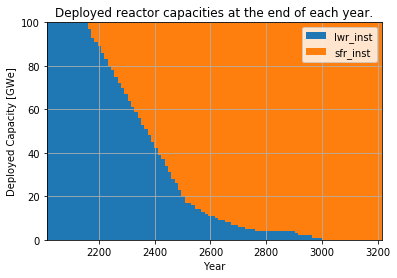
\includegraphics[scale=0.7]{./images/results_18/power_plot.png}
	\end{center}
	\caption{Deployed reactor capacities at the end of each year from Cyclus.}
	\label{fig:pow_plot}
\end{figure}


\begin{figure}[htbp!]
	\begin{center}
		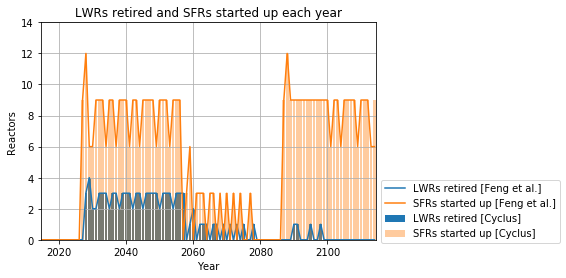
\includegraphics[scale=0.7]{./images/results_18/dep.png}
	\end{center}
	\caption{\glspl{LWR} retired and \glspl{SFR} started up each year.}
	\label{fig:dep}
\end{figure}

Figure \ref{fig:fuel_load} shows the annual fuel loading rate.
The initial fuel loading for 100 \gls{LWR} reactors are not shown in
the plot for both the benchmark and the Cyclus results.
The oscillations caused by the 18 month refueling period
were aggregated into 12 month groups. As a result the total fuel loaded
is equal for both plots.

Although indistinguishable in figure \ref{fig:fuel_load},
there is a small difference between \gls{SFR} fuel loading proportional
to the core mass difference, because Cyclus only has integer batch numbers.
Figure \ref{fig:fuel_load_diff_norm} shows the
differences normalized by the core mass differences, overlapped with the
\gls{SFR} deployment. This shows that the differences only occur during
deployment due to the difference in core mass.


\begin{figure}[htbp!]
	\begin{center}
		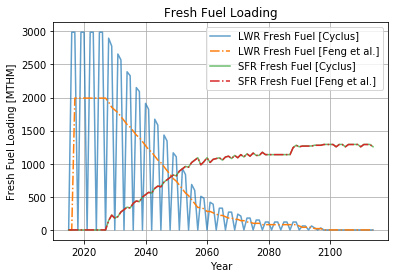
\includegraphics[scale=0.7]{./images/results_18/fuel_load.png}
	\end{center}
	\caption{Annual fresh fuel loading rates (first cores and reload fuel).}
	\label{fig:fuel_load}
\end{figure}

Figure \ref{fig:fuel_discharge_monthly} shows the inventory of discharged
\gls{UNF} in the mandatory cooling stage (four years for \gls{LWR}, one year for \gls{SFR}).
It also oscillates around the benchmark's
solution and converges, due to the influx and the outflux of \gls{UNF}
into and out of the storage facility.
The \gls{SFR} inventory and fuel loading
solutions exactly matches the benchmark solutions, minus the small ($1.07\%$) difference due to core
size.

\begin{figure}[htbp!]
	\begin{center}
		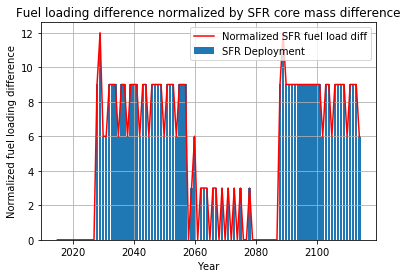
\includegraphics[scale=0.7]{./images/results_18/fuel_load_diff_norm.png}
	\end{center}
	\caption{Difference between annual fresh \gls{SFR} fuel loading rates (Cyclus - Benchmark) normalized by the core mass difference of an \gls{SFR} due to fractional batch size.}
	\label{fig:fuel_load_diff_norm}
\end{figure}


Figure \ref{fig:waiting_monthly} shows the amount of cooled \gls{UNF} waiting for
reprocessing. The value is calculated by subtracting the cumulative difference between
the cooled inventory and the \gls{UNF} reprocessing throughput.

\[ M_{wait, t} = M_{cooled, t} - M_{rep, t} \]

The oscillation is between the cooled inventory in the storage facility before (high)
and after (low) it sends its inventory for reprocessing.

\begin{figure}[htbp!]
	\begin{center}
		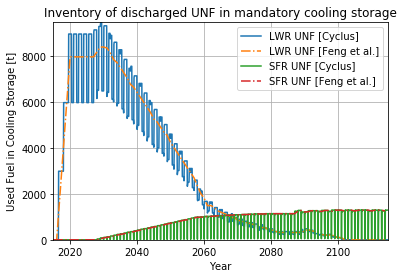
\includegraphics[scale=0.7]{./images/results_18/fuel_discharge_monthly.png}
	\end{center}
	\caption{Inventory of discharged \gls{UNF} in mandatory cooling storage.}
	\label{fig:fuel_discharge_monthly}
\end{figure}


\begin{figure}[htbp!]
	\begin{center}
		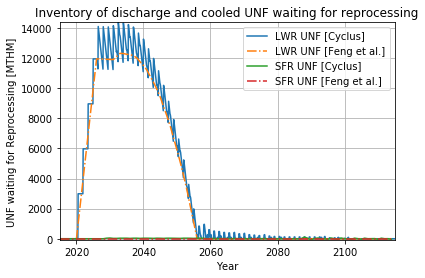
\includegraphics[scale=0.7]{./images/results_18/waiting_monthly.png}
	\end{center}
	\caption{Inventory of discharged and cooled \gls{UNF} waiting for reprocessing.}
	\label{fig:waiting_monthly}
\end{figure}


Figure \ref{fig:rep} shows the reprocessing throughput, which oscillates around
the benchmark solution. No oscillation exists from 2030 to 2055 because the
\gls{LWR} \gls{UNF} reprocessing plant throughput peaks at 2,000 tons per year.

\begin{figure}[htbp!]
	\begin{center}
		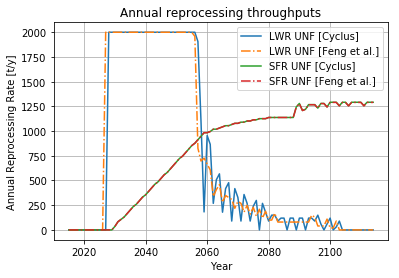
\includegraphics[scale=0.7]{./images/results_18/rep.png}
	\end{center}
	\caption{Annual reprocessing throughputs.}
	\label{fig:rep}
\end{figure}


Figure \ref{fig:tru} shows the inventory of unused \gls{TRU} recovered from \gls{UNF}.
The \Cyclus results follow the benchmark solutions closely. However,
the larger \gls{SFR} core size in Cyclus causes \Cyclus results to be 1.07\% smaller than the benchmark results,
since more \gls{TRU} is used to
start up the newly deployed \glspl{SFR}.

\begin{figure}[htbp!]
	\begin{center}
		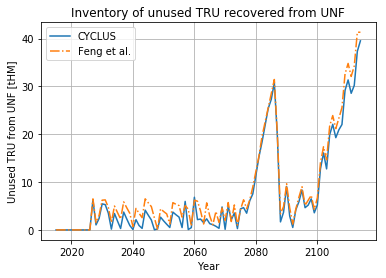
\includegraphics[scale=0.7]{./images/results_18/tru.png}
	\end{center}
	\caption{Inventory of unused \gls{TRU} recovered from \gls{UNF}.}
	\label{fig:tru}
\end{figure}

\section{Discussion}

We verified \Cyclus with results from an established
verification study and saw good agreement
in a transition scenario.

Throughout this work, two major differences were identified
that led to the deviation
of \Cyclus results from that of the benchmark solution. First,
the \Cycamore reactor depletes only half of its core
when decommissioned. Second, \Cyclus, unlike other
codes examined in the benchmark (except ORION), fully resolves
discrete batches for fuel discharge.
We resolve the first discrepancy by changing one line in the Cycamore source code.

This study proves that \Cyclus is a capable tool for modeling
fuel cycle transition scenarios.